\label{hwdriver}
This section will describe step by step how to write an hardware endpoint.
You will be required to write your own endpoint in case non of the existing endpoints
matches your hardware.

First let's have a look at how EFSL is structured internally.\\\\
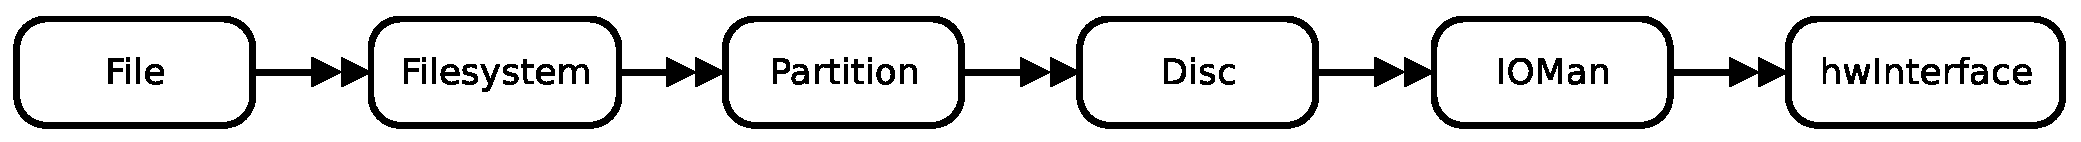
\includegraphics[scale=0.4]{schematics/objectmodel.eps}\\

As you can see we have created a linear object model that is quite simple.
The file en filesystem object deal with handling the filesystem specific stuff.
Below that we find the Partition object that is responsible for translating partition
relative addressing into disc-based LBA addressing.

The Disc object hold the partition table, and has a direct link to a cache manager, IOMan.
In IOMan, all requests for disc sectors come together. IOMan will perform checks to see
if sectors have to be read from disc (or from memory), or written back to disc.
In the latter case (reading or writing to disc), a request is made to the hardware layer.

The hardware interface has 3 responsibilities :
\begin{itemize}
	\item Initialize the hardware
	\item Read sectors from disc
	\item Write sectors to disc
\end{itemize}

All requests are \textsl{sector}based, a sector is a 512 byte piece from the disc, that is aligned to
a 512 byte boundary.\\\\
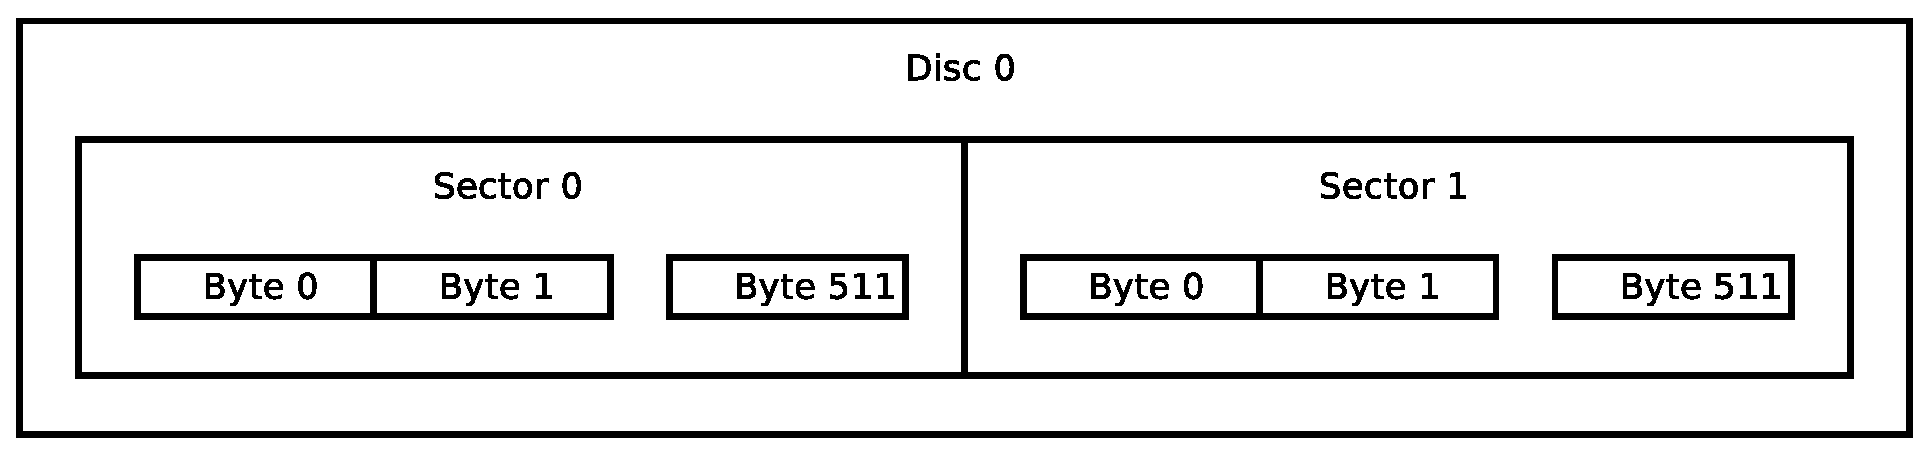
\includegraphics[scale=0.4]{schematics/sector.eps}

In this example we will create a new endpoint that will add support for data over pigeon carrier
for the EFSL. Initializing the hardware will require feeding the pigeon and telling it where the
data is. Reading/Writing will entail giving the bird the sector and letting it fly.

Perform the following steps:
\begin{enumerate}

	\item Choose a name for your endpoint\\
	You will need this name to create the required defines in the source code.
	For our example I've chosen the name \code{PIGEON\_CARRIER}.
	For consistency the final name is then \code{HW\_ENDPOINT\_PIGEON\_CARRIER}.

	\item Verify the sizes of integers\\
	Open \filename{inc/types.h} and create a new entry for pigeon carriers. Perhaps
	one of the existing sets is identical to yours and you can copy-paste it.

	\item Add your endpoint to \filename{interface.h}\\
	Locate the file \filename{interface.h} located in the directory \filename{inc/}
	Add a pigeon entry (located above the \code{\#else ... NO INTERFACE DEFINED})
\begin{lstlisting}
#if defined(HW_ENDPOINT_0)
   		#include "interfaces/0.h"
#elif defined(HW_ENDPOINT_1)
        #include "interfaces/1.h"
#elif defined(HW_ENDPOINT_PIGEON_CARRIER)
        #include "interfaces/pigeon.h"
#else
        #error "NO INTERFACE DEFINED - see interface.h"
#endif
\end{lstlisting}

	\item Select your endpoint in \filename{conf/config.h}
	
	\item Create your sourcefiles\\
	Create a header file in \filename{inc/} and a sourcefile in \filename {src/interfaces}.
	In this example I'm using \filename{pigeon.h} and \filename{pigeon.c}.

	\item Add your object file to the Makefile
	Take the Makefile that works best on your platform (they should all work with
	GNU/Make), or create a new one, using the existing one's as a template.
	Make sure to include your new pigeon object to the library.
	If you have an 'ar' like utility you can create a static library, else you may
	have to create a new project containing all required source files.

\end{enumerate}

The basic framework is now complete, now all that's left to do is to write the code
that will perform the actual flying work.

\subsubsection{hwInterface}
This structure represents the underlying hardware. There are some field that are required
to be present (because EFSL uses them), but you may put in as much or a little as
your driver requires to access the hardware.

As always in embedded design it is recommended to keep this structure as small
as possible.

Example:
\begin{lstlisting}
struct hwInterface{
	/* Field created for THIS hardware */
	Pigeon pigeon;

	/* Obligatory fields */
	euint32 sectorCount;
};
typedef struct hwInterface hwInterface;
\end{lstlisting}

\subsubsection{if\_initInterface}
This function will be called one time, when the hardware object is initialized 
by \code{efs\_init()}. This code should bring the hardware in a ready to use 
state.

The function's prototype is\\
\code{esint16 if\_initInterface(hwInterface *hw, euint8* opts);}

Optionally but recommended you should fill in the hw->sectorCount field with the number
of sectors. This field is used to validate sectorrequests.

An example of a initInterface function :
\begin{lstlisting}
esint16 if_initInterface(hwInterface *hw, euint8* opts)
{
	/* Parse options */
	parse_options(opts); /* Your application may not need options */

	/* Check hardware state */
	if(!alive(hw->pigeon)){
		//printf("Pigeon died! :-(\n");
		return(DEAD_PIGEON); /* #define DEAD_PIGEON -1 */
	}

	/* Initialize hardware */
	feed(hw->pigeon);
	pet (hw->pigeon);

	/* Get sectors count */
	hw->numSectors = ask_pigeon_num_sectors(hw->pigeon);

	return(0);
}
\end{lstlisting}

\subsubsection{if\_readBuf}
This function is responsible to read a sector from the disc and store it in a user supplied buffer. You will receive the hardware object, an address and a pointer to memory for storing
the buffer.

Please be very careful to respect the boundaries of the buffers, since it will usually be IOMan
calling this function, and if you have a buffer overflow you might corrupt the cache of the
the next buffer, which in turn may produce extremely rare and impossible to retrace behavior.

The function prototype is:\\
\code{esint16 if\_readBuf(hwInterface *hw,euint32 address, euint8* buf);}

The address is an LBA address, relative to the beginning of the disc. Should you be
accessing an old hard disc, or a device which uses some other form of addressing you will have to
recalculate the address to your own addressing scheme. Please note that there is no support
for sectors that are not 512 bytes large.

\begin{lstlisting}
esint8 if_readBuf(hwInterface* hw,euint32 address,euint8* buf)
{
	Message new_message;

	new_message.address = address;
	new_message.command = READ;

	pigeon_send(hw->pigeon,new_message); /* Launches the pigeon */
	while(!pigeon_returned(hw->pigeon)); /* Wait until the bird is back */
	memcpy(new_message.data,buf,512); /* Copy buffer */
	return(0);
}
\end{lstlisting}

\subsubsection{if\_writeBuf}
The function \code{if\_writeBuf} works exactly the same as it's reading variant.
